\documentclass[12pt,a4paper,german]{article}
\usepackage[utf8]{inputenc}
\usepackage[german]{babel}
\usepackage[T1]{fontenc}
\usepackage{amsmath}
\usepackage{amsfonts}
\usepackage{amssymb}
\usepackage[european, siunitx, strokediode]{circuitikz}
\usepackage{pgfplots} 
\usepackage{float}
\usepackage{fontspec}
\usepackage{tcolorbox}
\usepackage{fancyhdr}
\usepackage{titling}
\usepackage{csvsimple}
\usepackage{filecontents}
\usepackage{pdfpages}
\usepackage{listings}
\usepackage[left=2cm,right=2cm,top=2cm,bottom=2cm]{geometry}
\usepackage{titlesec}
\usepackage{lastpage}
\usepackage{tabularx}
\usepackage{svg}
\usepackage[framemethod=tikz]{mdframed}
\usepackage[iso]{isodate}
\usepackage[pdfauthor={tyrolyean},
            pdftitle={AQUADOC},
            pdfproducer={4BHN},
	    bookmarks=true,
            pdfcreator={xelatex}]{hyperref}
\usepackage{attachfile2}
\usepackage{xcolor}
\usepackage{fancyhdr}

\author{Manuel Ljubic, Jack Neuner, Daniel Plank}
\title{AquadDoc}
\setmainfont{Arial}

\pagestyle{fancy}
\fancyhf{}
\rhead{\thetitle}
\lhead{HN4-FTKL}
\cfoot{Seite \thepage von \pageref{LastPage}}
\rfoot{Ljubic, Plank, Neuner}
\lfoot{\dategerman{\today}}

\renewcommand{\headrulewidth}{.4mm}
\renewcommand{\footrulewidth}{.4mm}

\attachfilesetup{color=red}

% #############################################################################
% Compilation options. Used to enable or disable some parts of the document.
% #############################################################################

% Include the used datasheets in the document
\def\datasheets{0}

\def\psocdisasm{0}


\renewcommand{\headrulewidth}{.4mm}
\renewcommand{\footrulewidth}{.4mm}


% Define lst listing styles
\lstdefinestyle{customc}{
  belowcaptionskip=1\baselineskip,
  breaklines=true,
  frame=L,
  xleftmargin=\parindent,
  language=C,
  showstringspaces=false,
  keywordstyle=\bfseries\color{green!40!black},
  commentstyle=\itshape\color{purple!40!black},
  identifierstyle=\color{blue},
  stringstyle=\color{orange},
}

\lstdefinestyle{customasm}{
  belowcaptionskip=1\baselineskip,
  frame=L,
  xleftmargin=\parindent,
  language=[x86masm]Assembler,
  basicstyle=\footnotesize\ttfamily,
  commentstyle=\itshape\color{purple!40!black},
}

\lstset{escapechar=@,style=customc}

\begin{document}
\begin{titlepage}
\begin{center}
\setlength{\fboxrule}{1mm}
\framebox{

	\parbox{\textwidth}{
	
		\vspace{6mm}
		\centering
		\textbf{\Huge HN4-FTKL}
		\break
		\Large{
			Abteilung Elektronik \break
		}
		
		\normalsize{
			an der Höheren technischen Bundeslehranstalt 1 \break
			Innsbruck, Anichstraße 26 – 28 \break
		}
	}
}
\break
\vspace{1mm}
\setlength{\fboxrule}{.1mm}
\framebox{
	\parbox{\textwidth}{
		\textbf{\maketitle}
		\centering
		\textbf{Dokumentation des Wasserhaushalts einer 
	Wasserversorgungsanlage für Kleinsiedlungsgebiete}
		\vspace{1cm}
	}
}

\end{center}
\end{titlepage}

\tableofcontents
\newpage

\section{Aufgabenstellung}

\subsection{Aufbau}
\begin{figure}[H]
	\centering
	\def\svgwidth{\columnwidth}
	% Graphic for TeX using PGF
% Title: /home/tyrolyean/school/hwe/ftkl/aquadoc/aufbau.dia
% Creator: Dia v0.97.3
% CreationDate: Mon Jan 21 10:34:21 2019
% For: tyrolyean
% \usepackage{tikz}
% The following commands are not supported in PSTricks at present
% We define them conditionally, so when they are implemented,
% this pgf file will use them.
\ifx\du\undefined
  \newlength{\du}
\fi
\setlength{\du}{15\unitlength}
\begin{tikzpicture}
\pgftransformxscale{1.000000}
\pgftransformyscale{-1.000000}
\definecolor{dialinecolor}{rgb}{0.000000, 0.000000, 0.000000}
\pgfsetstrokecolor{dialinecolor}
\definecolor{dialinecolor}{rgb}{1.000000, 1.000000, 1.000000}
\pgfsetfillcolor{dialinecolor}
\pgfsetlinewidth{0.100000\du}
\pgfsetdash{}{0pt}
\pgfsetdash{}{0pt}
\pgfsetbuttcap
\pgfsetmiterjoin
\pgfsetlinewidth{0.100000\du}
\pgfsetbuttcap
\pgfsetmiterjoin
\pgfsetdash{}{0pt}
\definecolor{dialinecolor}{rgb}{1.000000, 1.000000, 1.000000}
\pgfsetfillcolor{dialinecolor}
\fill (6.632258\du,3.850000\du)--(6.632258\du,9.938333\du)--(12.524194\du,9.938333\du)--(12.524194\du,3.850000\du)--cycle;
\definecolor{dialinecolor}{rgb}{0.000000, 0.000000, 0.000000}
\pgfsetstrokecolor{dialinecolor}
\draw (6.632258\du,3.850000\du)--(6.632258\du,9.938333\du)--(12.524194\du,9.938333\du)--(12.524194\du,3.850000\du)--cycle;
\pgfsetbuttcap
\pgfsetmiterjoin
\pgfsetdash{}{0pt}
\definecolor{dialinecolor}{rgb}{0.000000, 0.000000, 0.000000}
\pgfsetstrokecolor{dialinecolor}
\draw (6.632258\du,3.850000\du)--(6.632258\du,9.938333\du)--(12.524194\du,9.938333\du)--(12.524194\du,3.850000\du)--cycle;
% setfont left to latex
\definecolor{dialinecolor}{rgb}{0.000000, 0.000000, 0.000000}
\pgfsetstrokecolor{dialinecolor}
\node at (9.578226\du,7.115417\du){Qulellfassung};
\pgfsetlinewidth{0.100000\du}
\pgfsetdash{}{0pt}
\pgfsetdash{}{0pt}
\pgfsetbuttcap
\pgfsetmiterjoin
\pgfsetlinewidth{0.100000\du}
\pgfsetbuttcap
\pgfsetmiterjoin
\pgfsetdash{}{0pt}
\definecolor{dialinecolor}{rgb}{1.000000, 1.000000, 1.000000}
\pgfsetfillcolor{dialinecolor}
\fill (22.250000\du,6.745000\du)--(22.250000\du,12.833333\du)--(28.141935\du,12.833333\du)--(28.141935\du,6.745000\du)--cycle;
\definecolor{dialinecolor}{rgb}{0.000000, 0.000000, 0.000000}
\pgfsetstrokecolor{dialinecolor}
\draw (22.250000\du,6.745000\du)--(22.250000\du,12.833333\du)--(28.141935\du,12.833333\du)--(28.141935\du,6.745000\du)--cycle;
\pgfsetbuttcap
\pgfsetmiterjoin
\pgfsetdash{}{0pt}
\definecolor{dialinecolor}{rgb}{0.000000, 0.000000, 0.000000}
\pgfsetstrokecolor{dialinecolor}
\draw (22.250000\du,6.745000\du)--(22.250000\du,12.833333\du)--(28.141935\du,12.833333\du)--(28.141935\du,6.745000\du)--cycle;
% setfont left to latex
\definecolor{dialinecolor}{rgb}{0.000000, 0.000000, 0.000000}
\pgfsetstrokecolor{dialinecolor}
\node[anchor=west] at (7.700000\du,11.650000\du){QF1};
% setfont left to latex
\definecolor{dialinecolor}{rgb}{0.000000, 0.000000, 0.000000}
\pgfsetstrokecolor{dialinecolor}
\node[anchor=west] at (23.750000\du,14.750000\du){BS1};
% setfont left to latex
\definecolor{dialinecolor}{rgb}{0.000000, 0.000000, 0.000000}
\pgfsetstrokecolor{dialinecolor}
\node[anchor=west] at (23.750000\du,16.513889\du){};
\pgfsetlinewidth{0.100000\du}
\pgfsetdash{}{0pt}
\pgfsetdash{}{0pt}
\pgfsetbuttcap
{
\definecolor{dialinecolor}{rgb}{0.000000, 0.000000, 0.000000}
\pgfsetfillcolor{dialinecolor}
% was here!!!
\pgfsetarrowsend{stealth}
\definecolor{dialinecolor}{rgb}{0.000000, 0.000000, 0.000000}
\pgfsetstrokecolor{dialinecolor}
\draw (12.524194\du,6.894167\du)--(22.250000\du,9.789167\du);
}
% setfont left to latex
\definecolor{dialinecolor}{rgb}{0.000000, 0.000000, 0.000000}
\pgfsetstrokecolor{dialinecolor}
\node[anchor=west] at (16.544526\du,7.431264\du){105m};
% setfont left to latex
\definecolor{dialinecolor}{rgb}{0.000000, 0.000000, 0.000000}
\pgfsetstrokecolor{dialinecolor}
\node at (25.195968\du,10.010417\du){Brunnenstube};
\pgfsetlinewidth{0.100000\du}
\pgfsetdash{}{0pt}
\pgfsetdash{}{0pt}
\pgfsetbuttcap
\pgfsetmiterjoin
\pgfsetlinewidth{0.100000\du}
\pgfsetbuttcap
\pgfsetmiterjoin
\pgfsetdash{}{0pt}
\definecolor{dialinecolor}{rgb}{1.000000, 1.000000, 1.000000}
\pgfsetfillcolor{dialinecolor}
\fill (47.200000\du,18.995000\du)--(47.200000\du,25.083333\du)--(53.091935\du,25.083333\du)--(53.091935\du,18.995000\du)--cycle;
\definecolor{dialinecolor}{rgb}{0.000000, 0.000000, 0.000000}
\pgfsetstrokecolor{dialinecolor}
\draw (47.200000\du,18.995000\du)--(47.200000\du,25.083333\du)--(53.091935\du,25.083333\du)--(53.091935\du,18.995000\du)--cycle;
\pgfsetbuttcap
\pgfsetmiterjoin
\pgfsetdash{}{0pt}
\definecolor{dialinecolor}{rgb}{0.000000, 0.000000, 0.000000}
\pgfsetstrokecolor{dialinecolor}
\draw (47.200000\du,18.995000\du)--(47.200000\du,25.083333\du)--(53.091935\du,25.083333\du)--(53.091935\du,18.995000\du)--cycle;
% setfont left to latex
\definecolor{dialinecolor}{rgb}{0.000000, 0.000000, 0.000000}
\pgfsetstrokecolor{dialinecolor}
\node at (50.145968\du,21.860417\du){Hauptbrunnen};
% setfont left to latex
\definecolor{dialinecolor}{rgb}{0.000000, 0.000000, 0.000000}
\pgfsetstrokecolor{dialinecolor}
\node at (50.145968\du,22.660417\du){};
\pgfsetlinewidth{0.100000\du}
\pgfsetdash{}{0pt}
\pgfsetdash{}{0pt}
\pgfsetbuttcap
{
\definecolor{dialinecolor}{rgb}{0.000000, 0.000000, 0.000000}
\pgfsetfillcolor{dialinecolor}
% was here!!!
\pgfsetarrowsend{stealth}
\definecolor{dialinecolor}{rgb}{0.000000, 0.000000, 0.000000}
\pgfsetstrokecolor{dialinecolor}
\draw (28.141935\du,9.789167\du)--(47.200000\du,22.039167\du);
}
% setfont left to latex
\definecolor{dialinecolor}{rgb}{0.000000, 0.000000, 0.000000}
\pgfsetstrokecolor{dialinecolor}
\node[anchor=west] at (36.750000\du,14.500000\du){200m-2km};
\pgfsetlinewidth{0.100000\du}
\pgfsetdash{}{0pt}
\pgfsetdash{}{0pt}
\pgfsetbuttcap
\pgfsetmiterjoin
\pgfsetlinewidth{0.100000\du}
\pgfsetbuttcap
\pgfsetmiterjoin
\pgfsetdash{}{0pt}
\definecolor{dialinecolor}{rgb}{1.000000, 1.000000, 1.000000}
\pgfsetfillcolor{dialinecolor}
\fill (64.075100\du,-9.367500\du)--(64.075100\du,-3.279167\du)--(69.967035\du,-3.279167\du)--(69.967035\du,-9.367500\du)--cycle;
\definecolor{dialinecolor}{rgb}{0.000000, 0.000000, 0.000000}
\pgfsetstrokecolor{dialinecolor}
\draw (64.075100\du,-9.367500\du)--(64.075100\du,-3.279167\du)--(69.967035\du,-3.279167\du)--(69.967035\du,-9.367500\du)--cycle;
\pgfsetbuttcap
\pgfsetmiterjoin
\pgfsetdash{}{0pt}
\definecolor{dialinecolor}{rgb}{0.000000, 0.000000, 0.000000}
\pgfsetstrokecolor{dialinecolor}
\draw (64.075100\du,-9.367500\du)--(64.075100\du,-3.279167\du)--(69.967035\du,-3.279167\du)--(69.967035\du,-9.367500\du)--cycle;
% setfont left to latex
\definecolor{dialinecolor}{rgb}{0.000000, 0.000000, 0.000000}
\pgfsetstrokecolor{dialinecolor}
\node at (67.021068\du,-6.102083\du){Qulellfassung};
\pgfsetlinewidth{0.100000\du}
\pgfsetdash{}{0pt}
\pgfsetdash{}{0pt}
\pgfsetbuttcap
\pgfsetmiterjoin
\pgfsetlinewidth{0.100000\du}
\pgfsetbuttcap
\pgfsetmiterjoin
\pgfsetdash{}{0pt}
\definecolor{dialinecolor}{rgb}{1.000000, 1.000000, 1.000000}
\pgfsetfillcolor{dialinecolor}
\fill (63.992842\du,0.627500\du)--(63.992842\du,6.715833\du)--(69.884777\du,6.715833\du)--(69.884777\du,0.627500\du)--cycle;
\definecolor{dialinecolor}{rgb}{0.000000, 0.000000, 0.000000}
\pgfsetstrokecolor{dialinecolor}
\draw (63.992842\du,0.627500\du)--(63.992842\du,6.715833\du)--(69.884777\du,6.715833\du)--(69.884777\du,0.627500\du)--cycle;
\pgfsetbuttcap
\pgfsetmiterjoin
\pgfsetdash{}{0pt}
\definecolor{dialinecolor}{rgb}{0.000000, 0.000000, 0.000000}
\pgfsetstrokecolor{dialinecolor}
\draw (63.992842\du,0.627500\du)--(63.992842\du,6.715833\du)--(69.884777\du,6.715833\du)--(69.884777\du,0.627500\du)--cycle;
% setfont left to latex
\definecolor{dialinecolor}{rgb}{0.000000, 0.000000, 0.000000}
\pgfsetstrokecolor{dialinecolor}
\node[anchor=west] at (59.892842\du,-3.567500\du){QF2};
% setfont left to latex
\definecolor{dialinecolor}{rgb}{0.000000, 0.000000, 0.000000}
\pgfsetstrokecolor{dialinecolor}
\node[anchor=west] at (60.392842\du,3.682500\du){BS2};
% setfont left to latex
\definecolor{dialinecolor}{rgb}{0.000000, 0.000000, 0.000000}
\pgfsetstrokecolor{dialinecolor}
\node[anchor=west] at (60.392842\du,5.446389\du){};
% setfont left to latex
\definecolor{dialinecolor}{rgb}{0.000000, 0.000000, 0.000000}
\pgfsetstrokecolor{dialinecolor}
\node at (66.938810\du,3.892917\du){Brunnenstube};
\pgfsetlinewidth{0.100000\du}
\pgfsetdash{}{0pt}
\pgfsetdash{}{0pt}
\pgfsetbuttcap
{
\definecolor{dialinecolor}{rgb}{0.000000, 0.000000, 0.000000}
\pgfsetfillcolor{dialinecolor}
% was here!!!
\pgfsetarrowsend{stealth}
\definecolor{dialinecolor}{rgb}{0.000000, 0.000000, 0.000000}
\pgfsetstrokecolor{dialinecolor}
\draw (67.021068\du,-3.279167\du)--(66.938810\du,0.627500\du);
}
\pgfsetlinewidth{0.100000\du}
\pgfsetdash{}{0pt}
\pgfsetdash{}{0pt}
\pgfsetbuttcap
{
\definecolor{dialinecolor}{rgb}{0.000000, 0.000000, 0.000000}
\pgfsetfillcolor{dialinecolor}
% was here!!!
\pgfsetarrowsend{stealth}
\definecolor{dialinecolor}{rgb}{0.000000, 0.000000, 0.000000}
\pgfsetstrokecolor{dialinecolor}
\draw (66.938810\du,6.715833\du)--(53.091935\du,22.039167\du);
}
\pgfsetlinewidth{0.100000\du}
\pgfsetdash{}{0pt}
\pgfsetdash{}{0pt}
\pgfsetbuttcap
\pgfsetmiterjoin
\pgfsetlinewidth{0.100000\du}
\pgfsetbuttcap
\pgfsetmiterjoin
\pgfsetdash{}{0pt}
\definecolor{dialinecolor}{rgb}{1.000000, 1.000000, 1.000000}
\pgfsetfillcolor{dialinecolor}
\fill (71.082358\du,25.700000\du)--(71.082358\du,30.471667\du)--(75.700100\du,30.471667\du)--(75.700100\du,25.700000\du)--cycle;
\definecolor{dialinecolor}{rgb}{0.000000, 0.000000, 0.000000}
\pgfsetstrokecolor{dialinecolor}
\draw (71.082358\du,25.700000\du)--(71.082358\du,30.471667\du)--(75.700100\du,30.471667\du)--(75.700100\du,25.700000\du)--cycle;
\pgfsetbuttcap
\pgfsetmiterjoin
\pgfsetdash{}{0pt}
\definecolor{dialinecolor}{rgb}{0.000000, 0.000000, 0.000000}
\pgfsetstrokecolor{dialinecolor}
\draw (71.082358\du,25.700000\du)--(71.082358\du,30.471667\du)--(75.700100\du,30.471667\du)--(75.700100\du,25.700000\du)--cycle;
% setfont left to latex
\definecolor{dialinecolor}{rgb}{0.000000, 0.000000, 0.000000}
\pgfsetstrokecolor{dialinecolor}
\node at (73.391229\du,28.307083\du){Haushalt};
\pgfsetlinewidth{0.100000\du}
\pgfsetdash{}{0pt}
\pgfsetdash{}{0pt}
\pgfsetbuttcap
{
\definecolor{dialinecolor}{rgb}{0.000000, 0.000000, 0.000000}
\pgfsetfillcolor{dialinecolor}
% was here!!!
\definecolor{dialinecolor}{rgb}{0.000000, 0.000000, 0.000000}
\pgfsetstrokecolor{dialinecolor}
\draw (50.111277\du,25.133448\du)--(50.000100\du,35.050000\du);
}
\pgfsetlinewidth{0.100000\du}
\pgfsetdash{}{0pt}
\pgfsetdash{}{0pt}
\pgfsetbuttcap
{
\definecolor{dialinecolor}{rgb}{0.000000, 0.000000, 0.000000}
\pgfsetfillcolor{dialinecolor}
% was here!!!
\definecolor{dialinecolor}{rgb}{0.000000, 0.000000, 0.000000}
\pgfsetstrokecolor{dialinecolor}
\draw (50.050100\du,34.900000\du)--(86.700100\du,34.950000\du);
}
\pgfsetlinewidth{0.100000\du}
\pgfsetdash{}{0pt}
\pgfsetdash{}{0pt}
\pgfsetbuttcap
\pgfsetmiterjoin
\pgfsetlinewidth{0.100000\du}
\pgfsetbuttcap
\pgfsetmiterjoin
\pgfsetdash{}{0pt}
\definecolor{dialinecolor}{rgb}{1.000000, 1.000000, 1.000000}
\pgfsetfillcolor{dialinecolor}
\fill (80.550100\du,25.440000\du)--(80.550100\du,30.211667\du)--(85.167842\du,30.211667\du)--(85.167842\du,25.440000\du)--cycle;
\definecolor{dialinecolor}{rgb}{0.000000, 0.000000, 0.000000}
\pgfsetstrokecolor{dialinecolor}
\draw (80.550100\du,25.440000\du)--(80.550100\du,30.211667\du)--(85.167842\du,30.211667\du)--(85.167842\du,25.440000\du)--cycle;
\pgfsetbuttcap
\pgfsetmiterjoin
\pgfsetdash{}{0pt}
\definecolor{dialinecolor}{rgb}{0.000000, 0.000000, 0.000000}
\pgfsetstrokecolor{dialinecolor}
\draw (80.550100\du,25.440000\du)--(80.550100\du,30.211667\du)--(85.167842\du,30.211667\du)--(85.167842\du,25.440000\du)--cycle;
% setfont left to latex
\definecolor{dialinecolor}{rgb}{0.000000, 0.000000, 0.000000}
\pgfsetstrokecolor{dialinecolor}
\node at (82.718850\du,27.880656\du){Haushalt};
\pgfsetlinewidth{0.100000\du}
\pgfsetdash{}{0pt}
\pgfsetdash{}{0pt}
\pgfsetbuttcap
{
\definecolor{dialinecolor}{rgb}{0.000000, 0.000000, 0.000000}
\pgfsetfillcolor{dialinecolor}
% was here!!!
\pgfsetarrowsend{stealth}
\definecolor{dialinecolor}{rgb}{0.000000, 0.000000, 0.000000}
\pgfsetstrokecolor{dialinecolor}
\draw (73.391229\du,30.471667\du)--(73.350100\du,35.112500\du);
}
\pgfsetlinewidth{0.100000\du}
\pgfsetdash{}{0pt}
\pgfsetdash{}{0pt}
\pgfsetbuttcap
{
\definecolor{dialinecolor}{rgb}{0.000000, 0.000000, 0.000000}
\pgfsetfillcolor{dialinecolor}
% was here!!!
\pgfsetarrowsend{stealth}
\definecolor{dialinecolor}{rgb}{0.000000, 0.000000, 0.000000}
\pgfsetstrokecolor{dialinecolor}
\draw (82.858971\du,30.211667\du)--(82.850100\du,34.962500\du);
}
% setfont left to latex
\definecolor{dialinecolor}{rgb}{0.000000, 0.000000, 0.000000}
\pgfsetstrokecolor{dialinecolor}
\node[anchor=west] at (74.874028\du,13.102116\du){BS ... Brunnbenstube};
% setfont left to latex
\definecolor{dialinecolor}{rgb}{0.000000, 0.000000, 0.000000}
\pgfsetstrokecolor{dialinecolor}
\node[anchor=west] at (74.874028\du,14.692439\du){HB... Hauptbrunnen};
% setfont left to latex
\definecolor{dialinecolor}{rgb}{0.000000, 0.000000, 0.000000}
\pgfsetstrokecolor{dialinecolor}
\node[anchor=west] at (74.874028\du,16.282761\du){HH... Haushalt};
% setfont left to latex
\definecolor{dialinecolor}{rgb}{0.000000, 0.000000, 0.000000}
\pgfsetstrokecolor{dialinecolor}
\node[anchor=west] at (74.874028\du,17.873083\du){QF... Quellfassung};
\end{tikzpicture}


	\label{fig:schemaufb}
	

\end{figure}

Ein Hochbehälter hat ein Fassungsvermögen um 1 Tag Wasser speichern zu können
oder ein Feuer zu löschen.
\subsection{Sensoren}

\begin{itemize}
	\item{Wasser zwischen Quelle und Brunnen und Brunnen und Häuser} \\
	 Umsetzung mittels Rotor mit Magnet an einer Schaufel, welcher einen
	 REED-Kontakt schaltet. Aufgabe: Prellt dieser Schalter?
	 \begin{figure}[H]
		\centering
		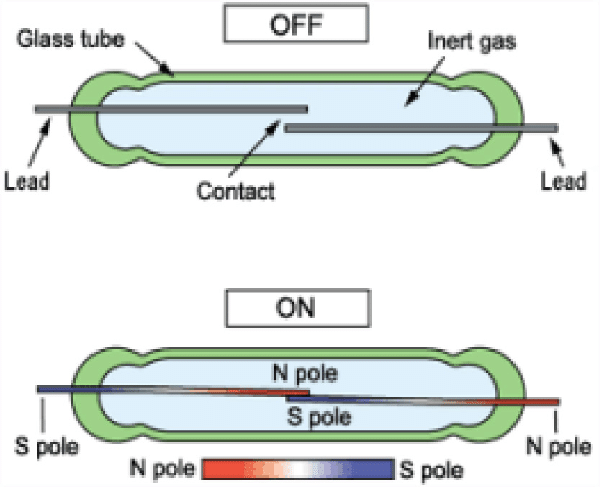
\includegraphics[width=0.5\textwidth]{Reed.png}
		\label{fig:reed}
		\caption{Schemata eines Reed-Schalters}
	\end{figure}

	\item{Wassertemperatur} \\
	Digitaler Sensor --> Auflösung von 0.01°C

	\item{Wasserstand}
	Füllstand HB: Drucksensor, Ultraschallsensor, Potentiometer mit
	Schwimmer, etc.

	\item{Türschalter}
	\item{Batteriestandsanzeige}


\end{itemize}

Anforderungen an die Funkübertragung:
\begin{itemize}
	\item{Datensicherheit}
	\item{Übertragungsmöglichkeit (Manchester Kodierung)}
	\item{Übertragungsantenne}
\end{itemize}

Gefundene Bauteile auf neuhold-elektronik.at:
\begin{itemize}
	\item{DS1722}: \\
	SPI Digital Thermometer. 8-12 bit Auflösung.
	
	\item{HC - SR04}: \\
	PWM Ultraschall Messmodul. 2mA standby strom.
	
	\item{MAX640}: \\
	5V Step-Down DC-DC Converter.

	
\end{itemize}

\section{Aufgabenverteilung}
\begin{itemize}
	\item{Plank: Programmentwicklung, testen der Sensoren und Teile der 
		Dokumentation}

	\item{Neuner: Programmentwicklung und erstellen des Top Design}

	\item{Ljubic: Dokumentation}
\end{itemize}

\subsection{Ljubic}

\begin{table}[H]
\centering 
\begin{tabularx}{\textwidth}{|l|X|l|}
\hline
\textbf{Datum} & \textbf{Beschreibung} & \textbf{Stunden} \\ 
\hline
\hline
04.02.19 & Aufgabenbesprechung & 3h \\ 
\hline
11.02.19 & Entfall & 0h \\ 
\hline
18.02.19 & Erstellen des Struktogramm  & 3h \\ 
\hline
25.02.19 & HC-SR04 Ultraschallsensor programmieren & 3h \\ 
\hline
04.03.19 & Dokumentation + Fertigstellen des Struktogramm & 3h \\ 
\hline
11.03.19 & Dokumentation & 3h \\ 
\hline
18.03.19 & Entfall & 0h\\ 
\hline
25.03.19 & Dokumentation + DS1722 Temperatursensor programmieren & 3h \\ 
\hline
01.04.19 & Dokumentation & 3h \\ 
\hline
08.04.19 & Dokumentation & 3h \\ 
\hline
29.04.19 & Dokumentation + Nachholen des Zeitplans & 3h \\ 
\hline
06.05.19 & Dokumentation + Einfügen der C-Codes in Dokumentation  & 3h \\ 
\hline
\hline
\end{tabularx}
\end{table}

\subsection{Neuner}

\begin{table}[H]
\centering 
\begin{tabularx}{\textwidth}{|l|X|l|}
\hline
\textbf{Datum} & \textbf{Beschreibung} & \textbf{Stunden} \\ 
\hline
\hline
04.02.19 & Aufgabenbesprechung & 3h \\ 
\hline
11.02.19 & Entfall & 0h \\ 
\hline
18.02.19 & Sensoren ausgewählt & 3h \\ 
\hline
25.02.19 & HC-SR04 Ultraschallsensor programmieren & 3h \\ 
\hline
04.03.19 & HC-SR04 Ultraschallsensor Verfeinerung & 3h \\ 
\hline
11.03.19 & DS1722 Temperatursensor programmieren & 3h \\ 
\hline
18.03.19 & Entfall & 0h\\ 
\hline
25.03.19 & Batteriestandmessung + DS1722 Temperatursensor programmieren & 3h \\ 
\hline
01.04.19 & DS1722 Temperatursensor programmieren& 3h \\ 
\hline
08.04.19 & DS1722 Temperatursensor programmieren & 3h \\ 
\hline
29.04.19 & BMP180 Temperatursensor programmieren & 3h \\ 
\hline
06.05.19 & BMP180 Temperatursensor programmieren & 3h \\ 
\hline
\hline
\end{tabularx}
\end{table}

\subsection{Plank}
\begin{table}[H]
\centering 
\begin{tabularx}{\textwidth}{|l|X|l|}
\hline
\textbf{Datum} & \textbf{Beschreibung} & \textbf{Stunden} \\ 
\hline
\hline
04.02.19 & Aufgabenbesprechung & 3h \\ 
\hline
11.02.19 & Frei & 0h \\ 
\hline
18.02.19 & Sensoren ausgewählt + Beginn der Dokumentation & 3h \\ 
\hline
25.02.19 & HC-SR04 Ultraschallsensor programmieren + Dokumentationserweiterung & 3h \\ 
\hline
04.03.19 & HC-SR04 Ultraschallsensor Verfeinerung& 3h \\ 
\hline
11.03.19 & DS1722 Temperatursensor programmieren & 3h \\ 
\hline
18.03.19 & Entfall & 0h\\ 
\hline
25.03.19 & DS1722 Temperatursensor programmieren & 3h \\ 
\hline
01.04.19 & DS1722 Temperatursensor programmieren & 3h \\ 
\hline
08.04.19 & DS1722 Temperatursensor programmieren & 3h \\ 
\hline
29.04.19 & BMP180 Temperatursensor programmieren & 3h \\ 
\hline
06.05.19 & DS1722 Temperatursensor programmieren & 3h \\ 
\hline
\hline
\end{tabularx}
\end{table}


\section{Test mittels Aurduino}

Es wird ein Arduino verwendet um die gegebenen Sensoren DS1722 bzw. HC-SR04 zu 
testen. Die SPI-Anschlüsse des Arduinos werden mit den Anschlüssen der
jeweiligen Sensoren verbunden ebenfalls wird auf die Verwendung der richtigen Versorgungsspannung geachtet.

\newpage
\subsection{HC-SR04}

\lstinputlisting[language=C++, numbers=left, frame=trBL, breaklines=true,
 breakautoindent=true, formfeed=\newpage, label={lst:ardu_hc-sr04},
 caption={Arduino Programm für HC-SR04}, columns=flexible]
 {./arduino/HC-SR04/HC-SR04.ino}

\newpage
\subsection{BMP180}

\lstinputlisting[language=C++, numbers=left, frame=trBL, breaklines=true,
 breakautoindent=true, formfeed=\newpage, label={lst:ardu_ds1722},
 caption={Arduino Programm für DS1722}, columns=flexible]
 {./arduino/DS1722/DS1722.ino}

\newpage
\section{Durchführung Mittels PSoC}

	Die Realisierung des Projektes mittels des PSoC Microcontrollers wurde
	vom Lehrer vorgegeben. Dafür wurden zuerst Einzelprogramme erstellt,
	um die gewünschten Funktionalitäten einzeln zu testen. Die
	Einzelprogramme sollten dann zu einem Gesamtprogramm zusammengeführt
	werden, welches volle Funktionalität bietet.

	Der verwendete Mikrocontroller ist der PSoC 5LP Bezeichner 
	CY8C5888LTI-LP097.

\subsection{Timer-Interrupt}

Zum testen des Timer interrupts wird innerhalb der ISR das pin\_val flag gesetzt,
welches innerhalb der main abgefragt und rückgesetzt wird. Die ISR muss so kurz
wie möglich gehalten werden, um die überlagerung mehrer Interrupts zu
verhindern.

\subsubsection{C-Code}

\lstinputlisting[language=C, numbers=left, frame=trBL, breaklines=true,
	breakautoindent=true, formfeed=\newpage, label={lst:psoc_timer_main},
	caption={Timer-Interrupt Haupt-Programm}, columns=flexible]
	{psoc/psoc/test-timer-interrupt.cydsn/main.c}
\lstinputlisting[language=C, numbers=left, frame=trBL, breaklines=true,
	breakautoindent=true, formfeed=\newpage, label={lst:psoc_timer_isrs},
	caption={Timer-Interrupt ISR}, columns=flexible]
	{psoc/psoc/test-timer-interrupt.cydsn/isrsc.c}


\subsubsection{Top-Sheet}
	 
 \begin{figure}[H]
	\centering
	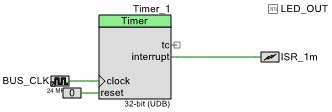
\includegraphics[width=\textwidth]{pictures/topsch_timer_int.png}
	\label{fig:topsch_timer_int}
	\caption{Top-Sheet des Timer-Interrupts}
\end{figure}

	
\subsection{Battery-Alarm}

\subsubsection{C-Code}

\lstinputlisting[language=C, numbers=left, frame=trBL, breaklines=true,
	breakautoindent=true, formfeed=\newpage, label={lst:psoc_battery_main},
	caption={Batteriestandmessung}, columns=flexible]
	{psoc/psoc/BatteryAlarmTestNeu.cydsn/Battery_Alarm.cydsn/main.c}

\subsubsection{Top-Sheet}
	 
 \begin{figure}[H]
	\centering
	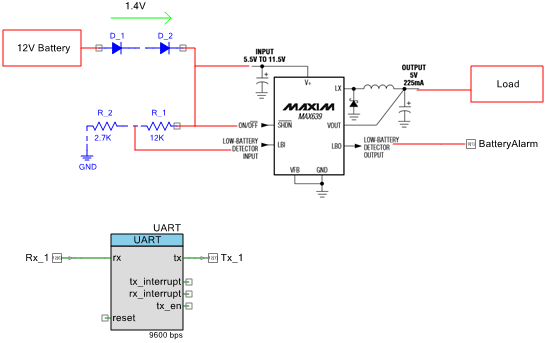
\includegraphics[width=\textwidth]{pictures/topsch_battery.png}
	\label{fig:topsch_batter}
	\caption{Top-Sheet des Batteriestandsmelder}
\end{figure}

\subsection{HC-SR04}

\subsubsection{Bauteilerklärung}
	
	Der HC-SR04 ist ein IC-Baustein, der Entfernung mittels Ultraschall
	misst. Dafür wird nach anlegen eines min. 10µs Pulses
	\footnote{Seite 2 HC-SR04 Datenblatt}
	am TRIG Pin
	ein Ultraschallimpuls losgeschickt. Der Baustein rechnet sich dann aus
	der Laufzeit des Impuls bis zu desen Rückkehr die Entfernung aus und
	gibt diese dann als PWM Signal am echo pin aus. Manche
	Module scheinen dabei einen Defekt zu haben oder schlichtweg billiger
	gebaut zu sein, da man bei diesen klar eine Kondensatorladekurve
	erkennen kann. Die Messergebnisse stimmen jedoch mit denen eines
	Funktionstüchtigen HC-SR04 überein, wenn man von CMOS Logikpegeln
	ausgeht, also 3.5V und höher
	\footnote{Halbleiter-Schaltungstechnik Seite 639} als 
	WAHR annimmt. Das HC-SR04 Datenblatt behaupt hierbei jedoch, dass die
	Logikpegel TTL-Pegel seien, was einen kleinen Offset in diesem Falle
	zur Folge hätte. Dieser konnte jedoch bei uns nicht gemessen werden.
	

	\begin{figure}[H]
		
		\centering
		\begin{tikzpicture}
		\begin{axis}[
			ylabel=$ Spannung $,
			xlabel=$ Zeit $,
			grid=both,
			minor tick num=5,
			width=\textwidth,
			height=0.5\textwidth,
			ymin = -0.1,
			ymax = 5.1,
			% If you want to make the lines thick
			%every axis plot/.append style={ultra thick},
			xmin = -0.00014,
			xmax = 0.0027
		]
		
		\addplot table [x=time, y=echo, col sep=comma, mark=none, 
			color=green] {measurements/hc-sr04_should.csv};
		\addplot table [x=time, y=trig, col sep=comma, mark=none, 
			color=red] {measurements/hc-sr04_should.csv};
		
		\end{axis}
		\end{tikzpicture}
		\label{fig:hc-sr04_working}

		\caption{Messung mit einem funktionstüchtigen HC-SR04}
	\end{figure}
	
	\begin{figure}[H]
		
		\centering
		\begin{tikzpicture}
		\begin{axis}[
			ylabel=$ Spannung $,
			xlabel=$ Zeit $,
			width=\textwidth,
			height=0.5\textwidth,
			ymin = -0.1,
			ymax = 5.1,
			% If you want to make the lines thick
			%every axis plot/.append style={ultra thick},
			xmin = -0.00014,
		]
		
		\addplot table [x=time, y=echo, col sep=comma, mark=none, 
			color=green] {measurements/hc-sr04_fail.csv};
		\addplot table [x=time, y=trig, col sep=comma, mark=none, 
			color=red] {measurements/hc-sr04_fail.csv};
		
		\end{axis}
		\end{tikzpicture}
		\label{fig:hc-sr04_broken}

		\caption{Messung mit einem sich nicht normal verhaltenden 
			HC-SR04}
	\end{figure}

	Die gemessene Pulslänge in ms soll durch 57 dividiert werden um den
	Abstand in cm zu erhalten.
	
\subsubsection{C-Code}
	
	Programm für den Ultraschallsensor zur Messung des Wasserstands im 
	Hochbehälter

	\lstinputlisting[language=C, numbers=left, frame=trBL, breaklines=true,
	breakautoindent=true, formfeed=\newpage, label={lst:psoc_hc-sr04},
	caption={PSoC funktionen für HC-SR04}, columns=flexible]
	{psoc/psoc/Ultrasonic_test.cydsn/hcsr04.c}
\subsubsection{Top-Sheet}
	 
	\begin{figure}[H]
		\centering
		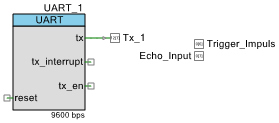
\includegraphics[width=\textwidth]{pictures/topsch_ultrasonic.png}
		\label{fig:topsch_ultrasonic}
		\caption{Top-Sheet der Wasserstandsmessung}
	\end{figure}

	
\subsection{Durchflussmessung}

\subsubsection{Bauteilerklärung}

Die Messung des Wasserdurchflusses wird mittels eines Standard Wasserzählers
durchgeführt. In diesem befindet sich ein Reed-Schalter welcher bei jeder vollen
Umdrehung des sich im Zählerbefindenden Schaufelrades einman betätigt wird. Dies
entspricht einem dem Datenblatt entnehmbaren Volumen an Wasser. In userem Falle
konnte jedoch kein Datenblatt aufgefunden Werden, anstelle dessen, war jedoch
die Menge an Wasser pro Impuls am Gerät selbst angeschrieben.


	\begin{figure}[H]
		\centering
		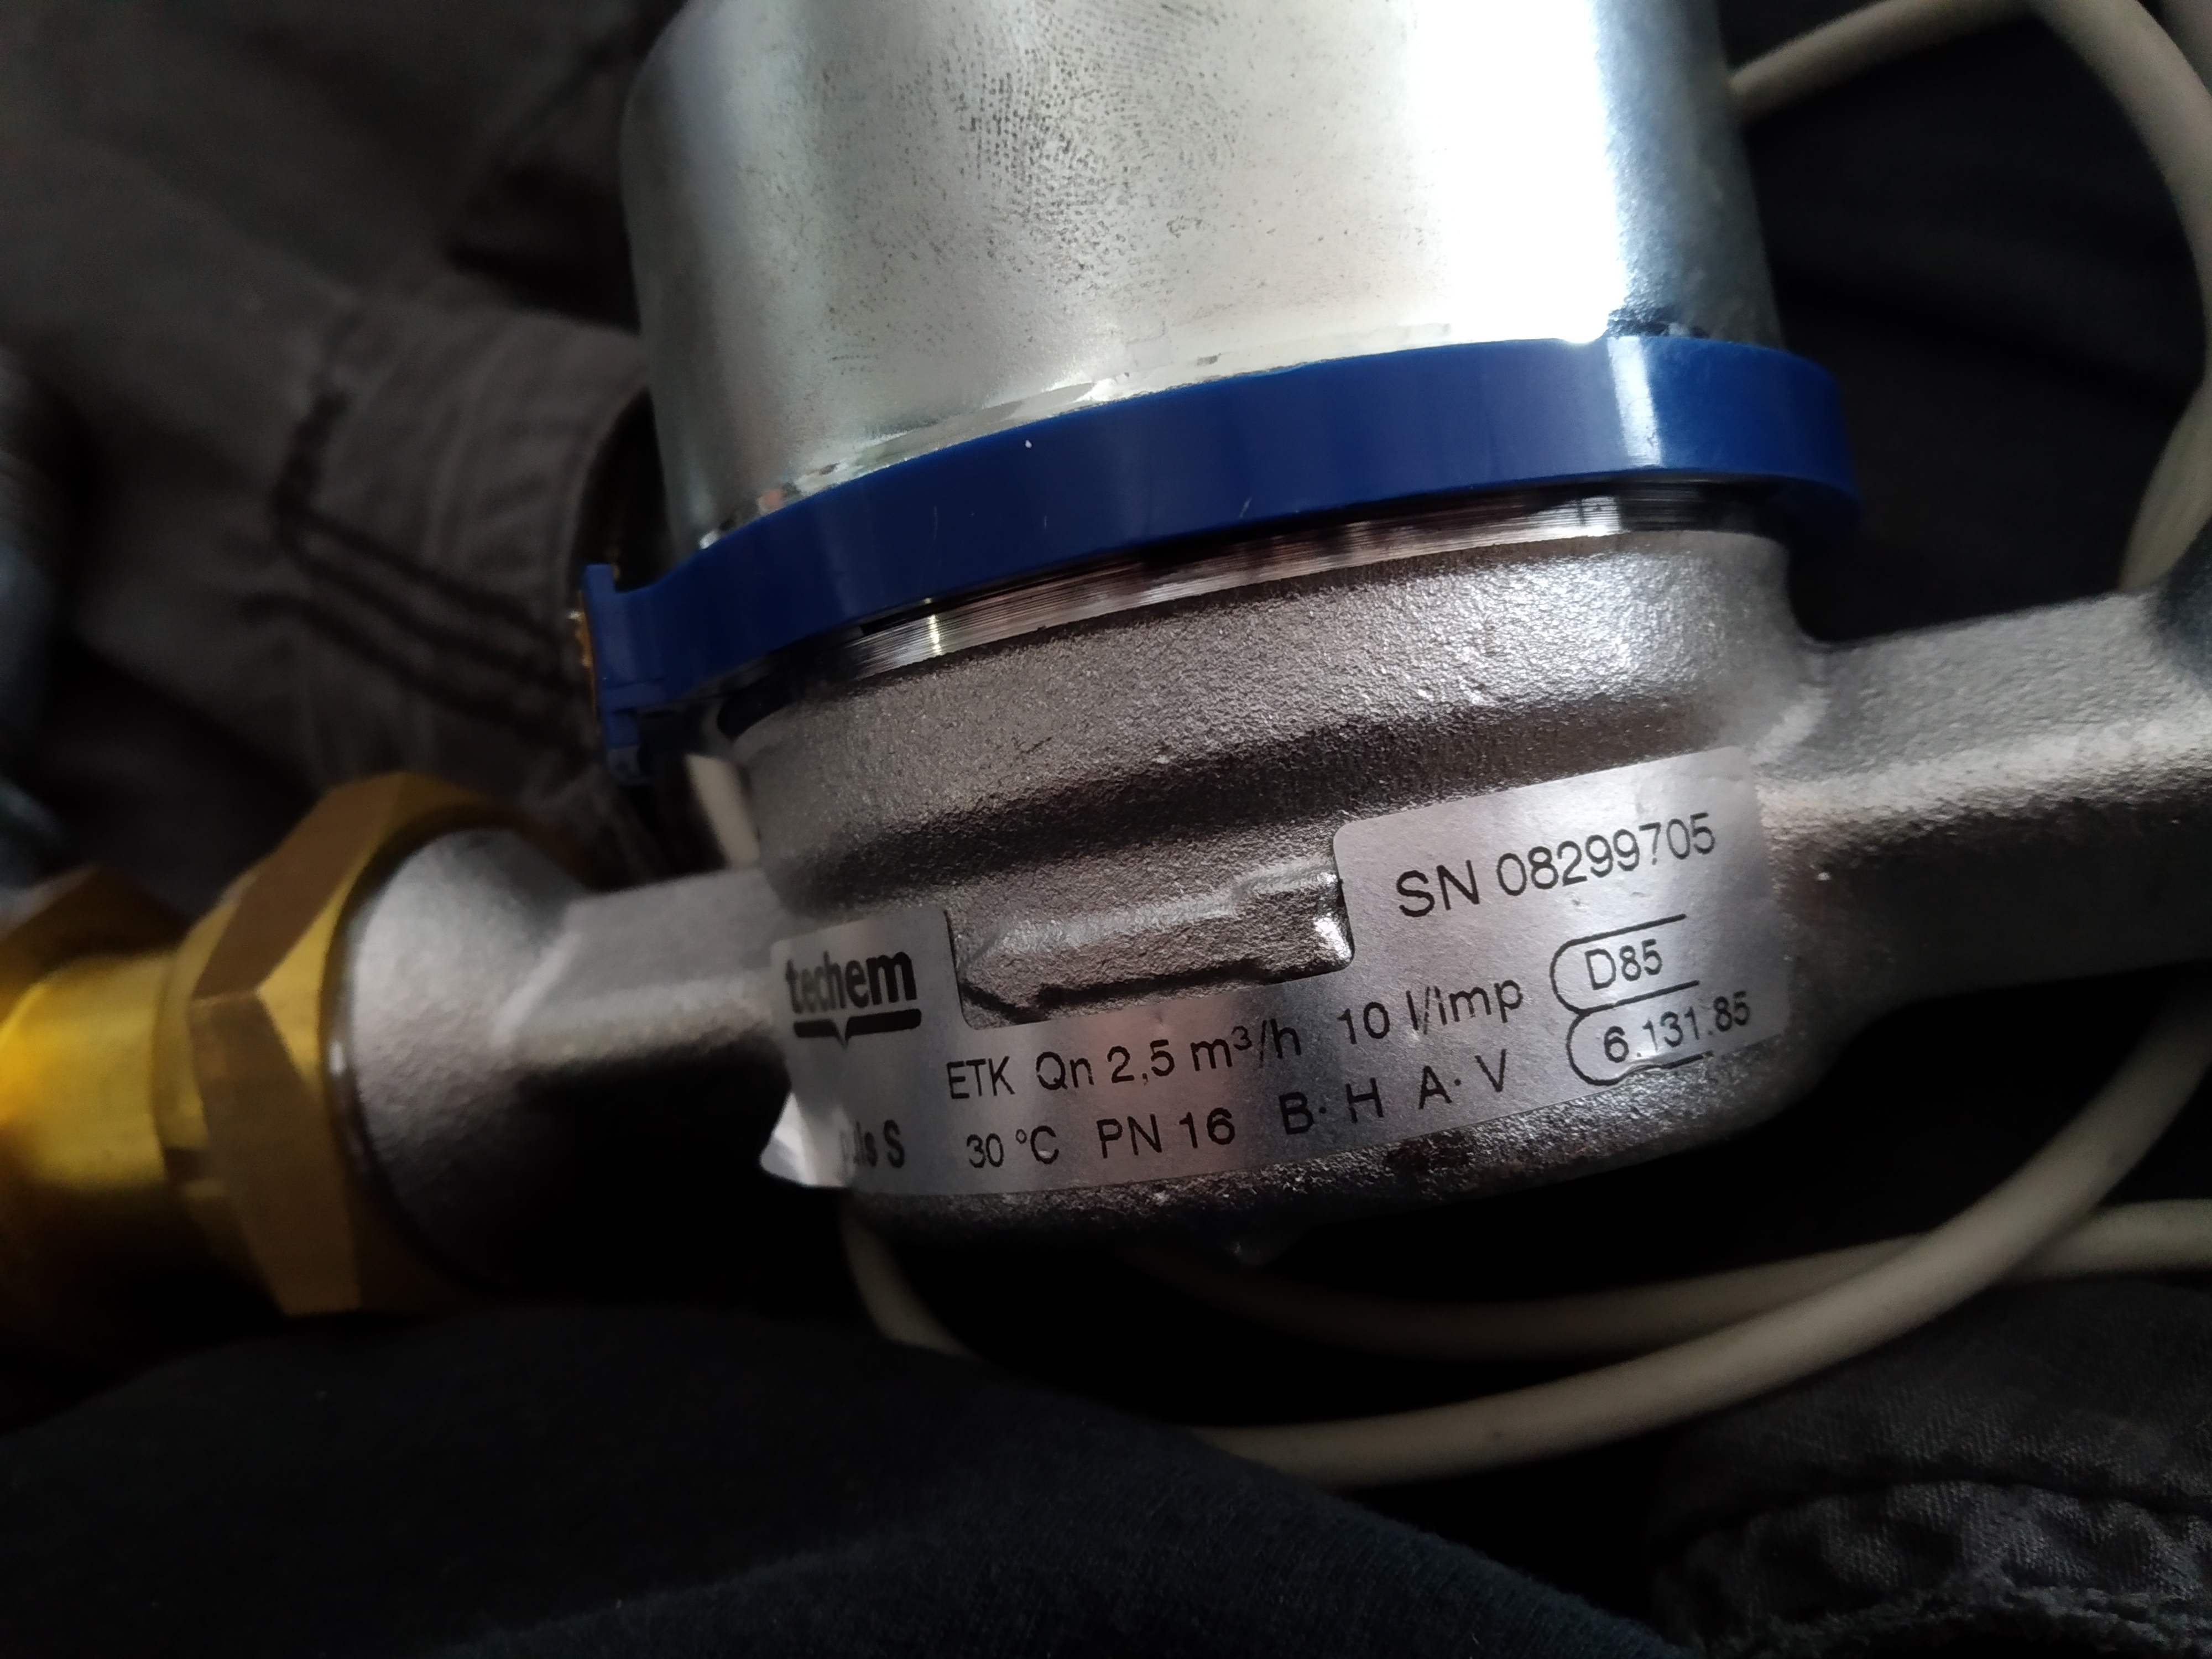
\includegraphics[width=\textwidth]{pictures/wasserzaehler.jpg}
		\label{fig:counter_hw}
		\caption{Der Wasserzähler}
	\end{figure}

\subsubsection{Prellen des REED-Kontaktes}

Da der Reed-Schalter ein physischer Schalter ist, welcher ein zwei Metallische
Oberflächen aufeinander aufschlagen lässt entsteht ein Schalter-Prellen.
Mithilfe des AnalogDiscoverys wurde versucht das Schalterprellen zu ermittlen,
wie man in dder Grafik \ref{fig:prellen} erkennen kann prellt der Schalter
nicht merklich, weshalb auf ein Entprellen mittles Kondensator, oder in Software
verzichtet wurde.

\begin{figure}[H]
	
	\centering
	\begin{tikzpicture}
	\begin{axis}[
		ylabel=$ Spannung $,
		xlabel=$ Zeit $,
		width=\textwidth,
		height=0.5\textwidth,
		xmin=-0.17,
		xmax=-0.14
		% If you want to make the lines thick
		%every axis plot/.append style={ultra thick},
	]
	
	\addplot table [x=t, y=u, col sep=comma, mark=none, 
		color=blue] {measurements/Reeeeeed_Schalter.csv};
	
	\end{axis}
	\end{tikzpicture}
	\label{fig:prellen}

	\caption{Messung des Schalterprellens mithilfe des Analog-Discovery}
\end{figure}


\subsubsection{C-Code}

\lstinputlisting[language=C, numbers=left, frame=trBL, breaklines=true,
	breakautoindent=true, formfeed=\newpage, 
	label={lst:psoc_waterflow_main},
	caption={Durchflussmessung}, columns=flexible]
	{psoc/psoc/water_flow.cydsn/main.c}

\subsubsection{Top-Sheet}
	 
	\begin{figure}[H]
		\centering
		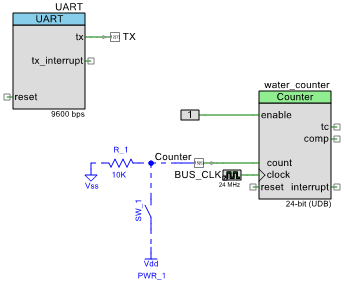
\includegraphics[width=\textwidth]{pictures/topsch_watercount.png}
		\label{fig:topsch_watercount}
		\caption{Top-Sheet de Wasserdurchflussmessung}
	\end{figure}

\newpage
\subsection{DS1722}

	Der DS1722 ist ein digitaler Temeperatur-Mess-IC von MAXIM Integrated.
	Er hat einen Messbereich von -60°C bis +120°C welchen er wahlweise mit
	8, 9, 10, 11 oder 12 bit auflösen kann. Als Schnittstellen hat er
	wahlweise 3-Wire oder SPI.
	\footnote{Serial Peripherial Interface, Standart von Motorola}. Welches
	Protokoll verwendet wird ist abhängig vom Spannungspegel am SERMODE
	Pin. Wenn am SERMODE Pin 5V anliegen, wird SPI verwendet, wenn 0V
	anliegen wird 3-Wire verwendet, den Pin nicht zu verbinden führt zu einem
	undefiniertem Verhalten.

	Im SPI-Modus werden die Pins SDI (Serial Data In) zu MOSI 
	(Master Output Slave Input) und SDO (Serial Data Out) zu MISO
	(Master Input Slave output). Der Chip-Enable Eingang
	\footnote{Der CE-Pin wird manchmal auch SS (Slave Slect) bezeichnet}
	ist HIGH-Aktiv, was im PSoC ein vorschalten eines Inverters vor den 
	CE-Pin erforderlich macht.

	Aufgrund anfänglicher Probleme mit dem PSoC wurde die Machbarkeit
	mittels ATMega nochmals überprüft. Dafür wurde eine ATMega2560
	als SPI Master verwendet, auf welchem die SPI-Pins in der GPIO-Bank B
	sind. Abbildung \ref{fig:spi_frame_atmega} zeigt einen mittels ATMega
	2560 erzeugten Datenverkehr mit dem DS1722.
	
	 
	 \begin{figure}[H]
		\centering
		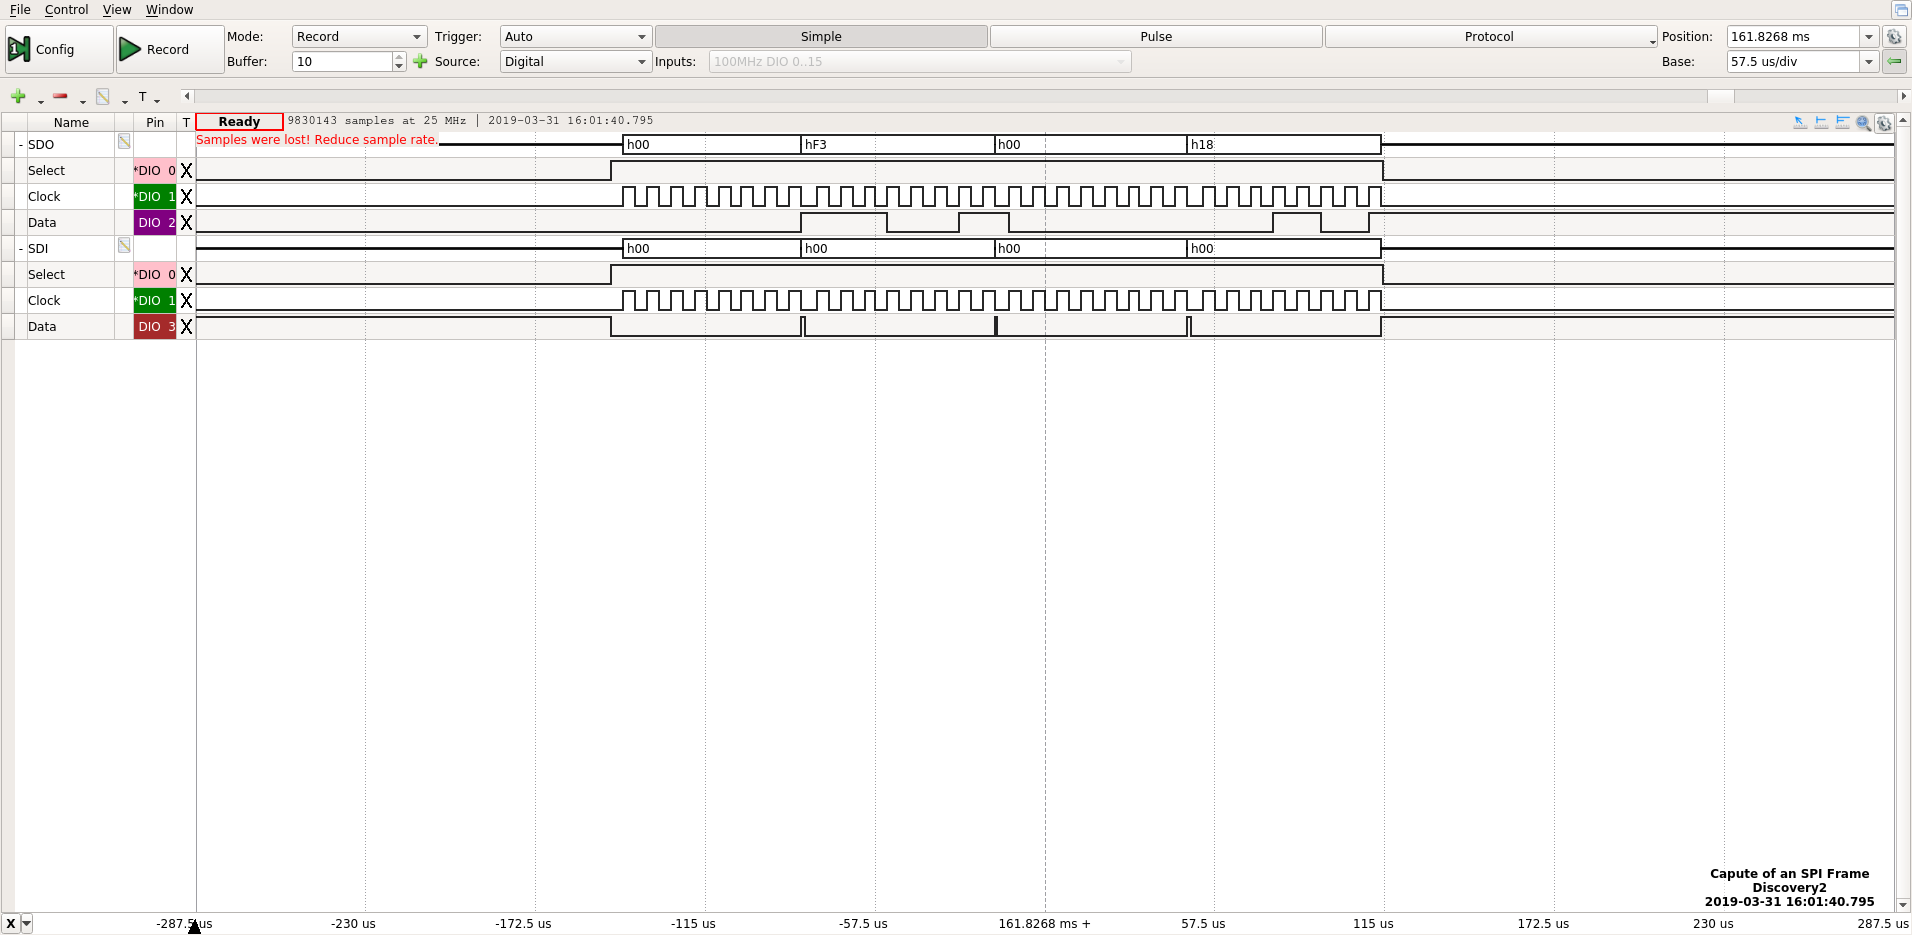
\includegraphics[width=1\textwidth]
			{measurements/spi_frame_recv_atmega}
		\label{fig:spi_frame_atmega}
		\caption{Erzielltes Ergebnis mit ATMega 2560}
	\end{figure}

	Die oben dargestellte Datensequenzentspricht erwarteten Werten. Die
	funktionstüchtigkeit des Sensors wurde dadurch bestätigt, und die
	Umsetzung mittels PSoC wurde erneut in angriff genommen. Die Temperatur-
	Messung mittels des Codes in Listing \ref{lst:psoc_ds1722} ist der
	aktuelle Stand.
\newpage
\subsubsection{C-Code für DS1722}

\lstinputlisting[language=C, numbers=left, frame=trBL, breaklines=true,
	breakautoindent=true, formfeed=\newpage, label={lst:psoc_ds1722},
	caption={Fehlerhaftes Temperaturmessungsprogramm für den DS1722}, 
	columns=flexible]
	{psoc/psoc/ds1722_test.cydsn/main.c}

\subsubsection{Top-Sheet}
	 
 \begin{figure}[H]
	\centering
	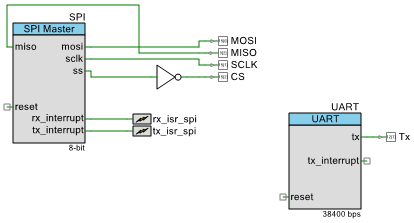
\includegraphics[width=0.5\textwidth]{pictures/topsch_ds1722.png}
	\label{fig:topsch_ds1722}
	\caption{Top-Sheet der Aktuellen DS1722 Schaltung}
\end{figure}

\section{Anhang}

\subsection{Literaturverzeichnis}

\begin{itemize}
	
	\item{\textbf{HC-SR04 Datenblatt}}\\
		Erhalten von mouser.com am 2019-03-10.
	\item{\textbf{DS1722 Datenblatt}}\\
		Erhalten von maximintegrated.com am 2019-03-10.
	\item{\textbf{MAX640 Datenblatt}}\\
		Erhalten von maximintegrated.com am 2019-03-10.
	\item{\textbf{CY8C5888LTI-LP097 Datenblatt}}\\
		Erhalten von cypress.com am 2019-03-10.
	\item{\textbf{Ulrich Tietze Christoph Schenk 
		Halbleiter-Schaltungstechnik}}\\
		Vorliegend in 12. Auflage Springer-Verlag Berlin Heidelberg 2002
	\item{\textbf{BIM-2 Datenblatt}}\\
		Erhalten von radiometrix.com 2019-05-06.

\end{itemize}

\if\datasheets1
	Die Angeführten Datenblätter wurden dem Dokument am Ende beigefügt.
\fi

\if\datasheets1
\subsection{Datenblätter}

	\subsubsection{HC-SR04}
	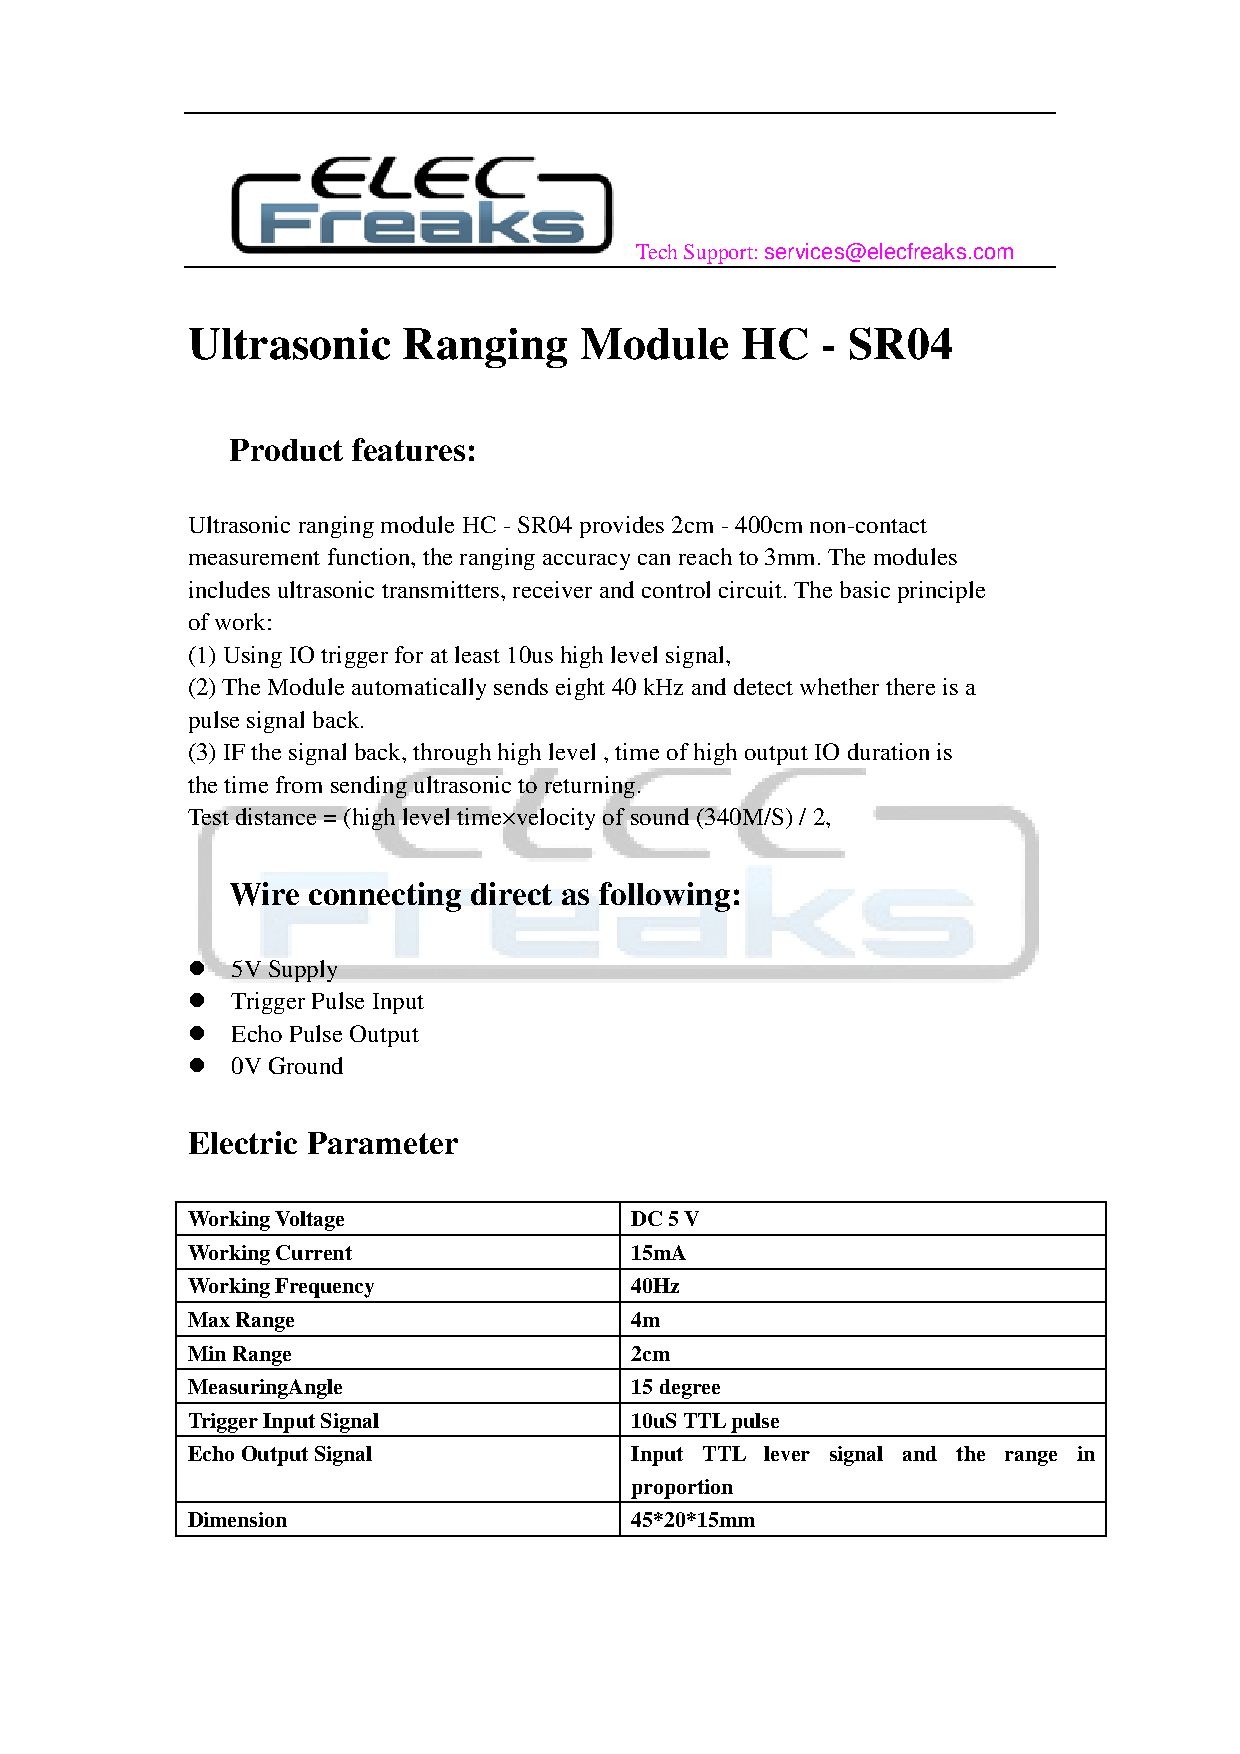
\includepdf[pages={1-}]{./datasheets/HCSR04-1022824.pdf}

	\subsubsection{DS1722}
	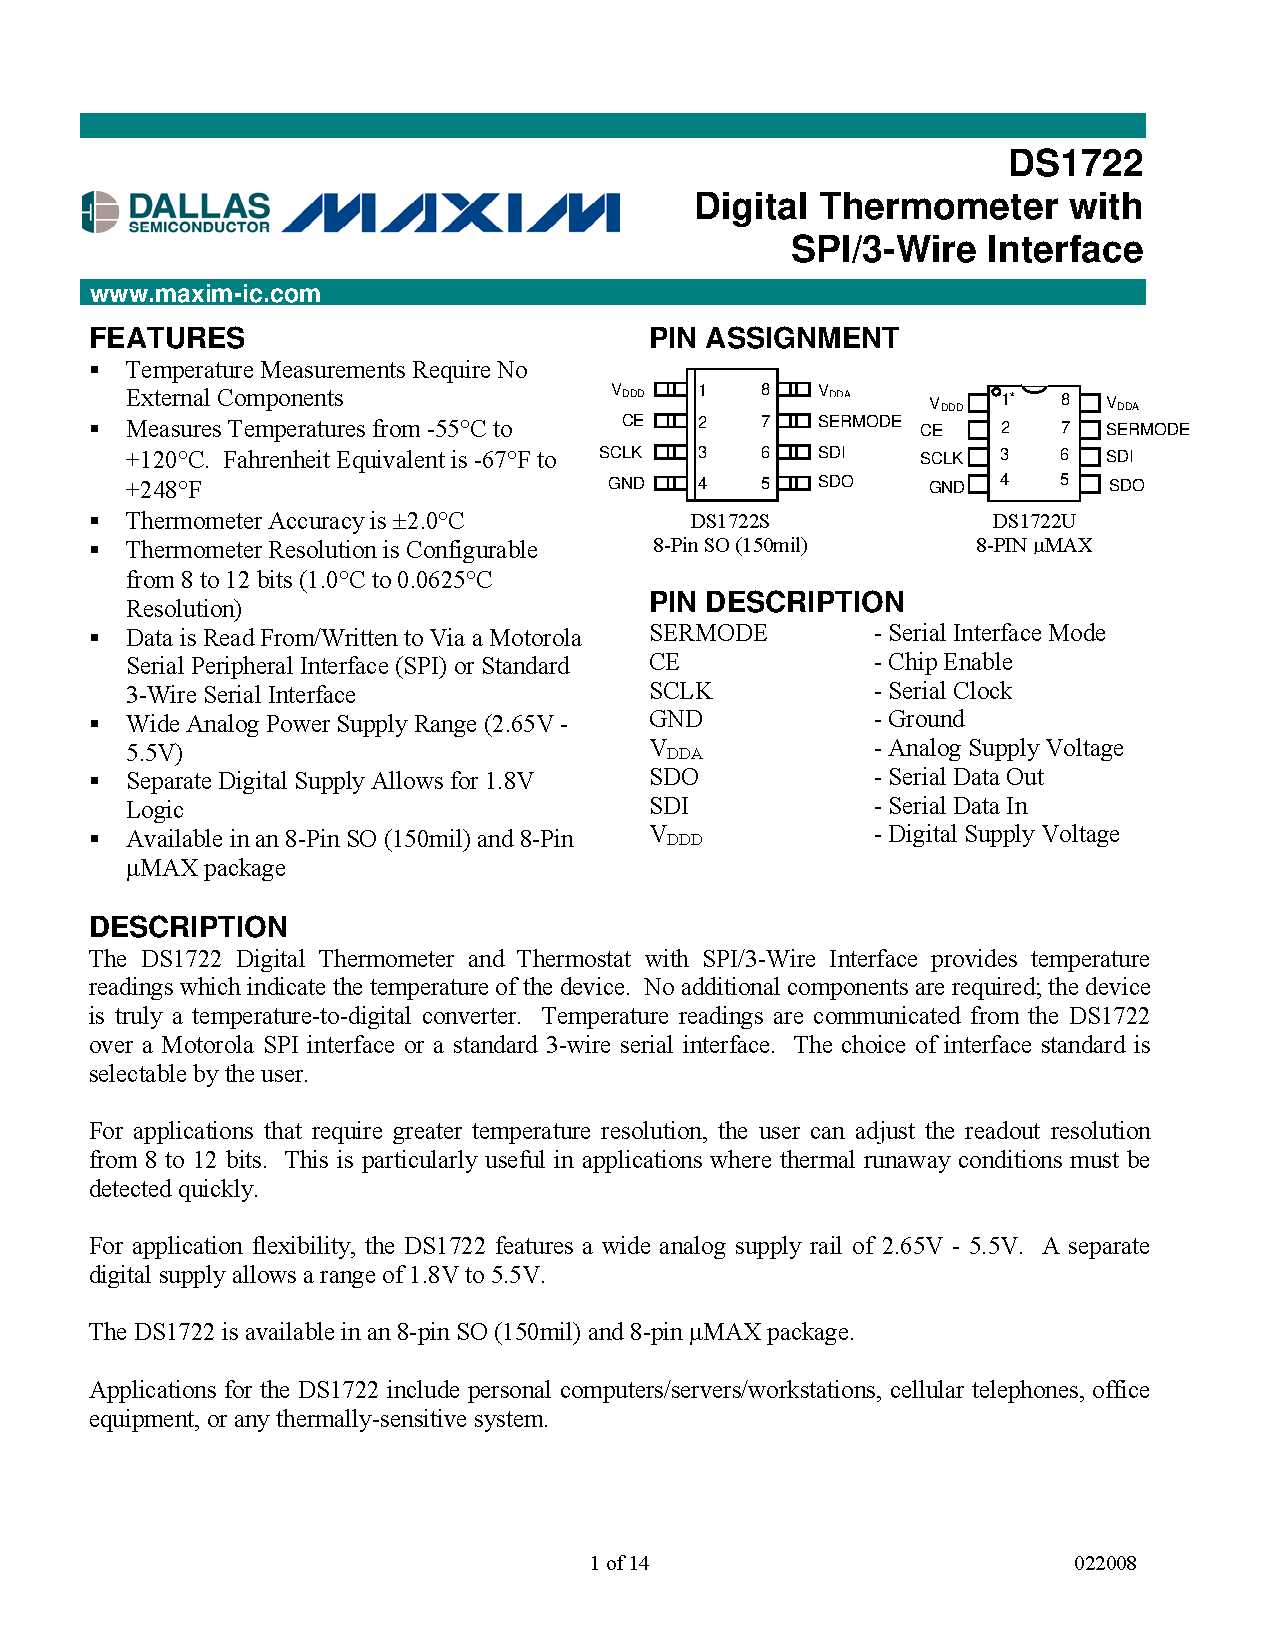
\includepdf[pages={1-}]{./datasheets/DS1722.pdf}

	\subsubsection{MAX640}
	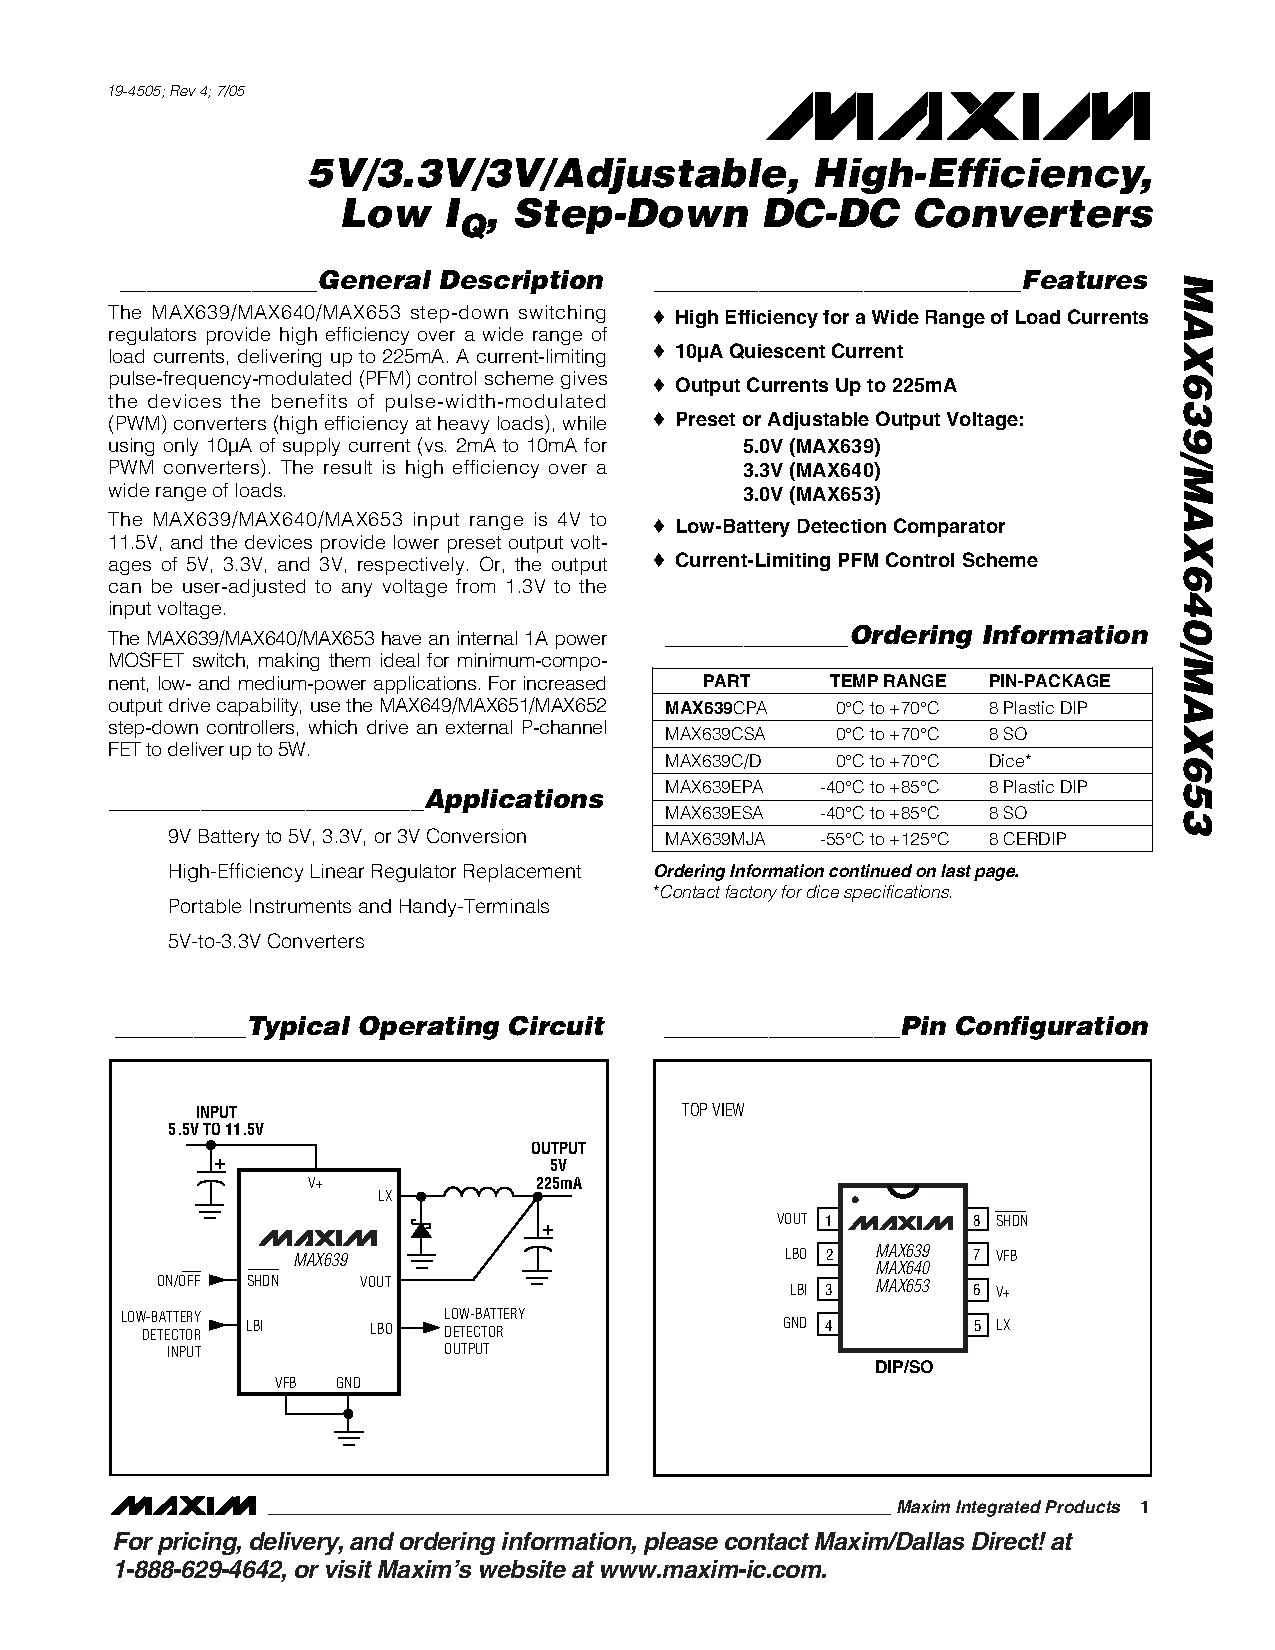
\includepdf[pages={1-}]{./datasheets/MAX639-MAX653.pdf}

	\subsubsection{CY8C5888LTI-LP097}
	\includepdf[pages={1-}]{./datasheets/CY8C5888LTI-LP097.pdf}
	
	\subsubsection{BIM-2}
	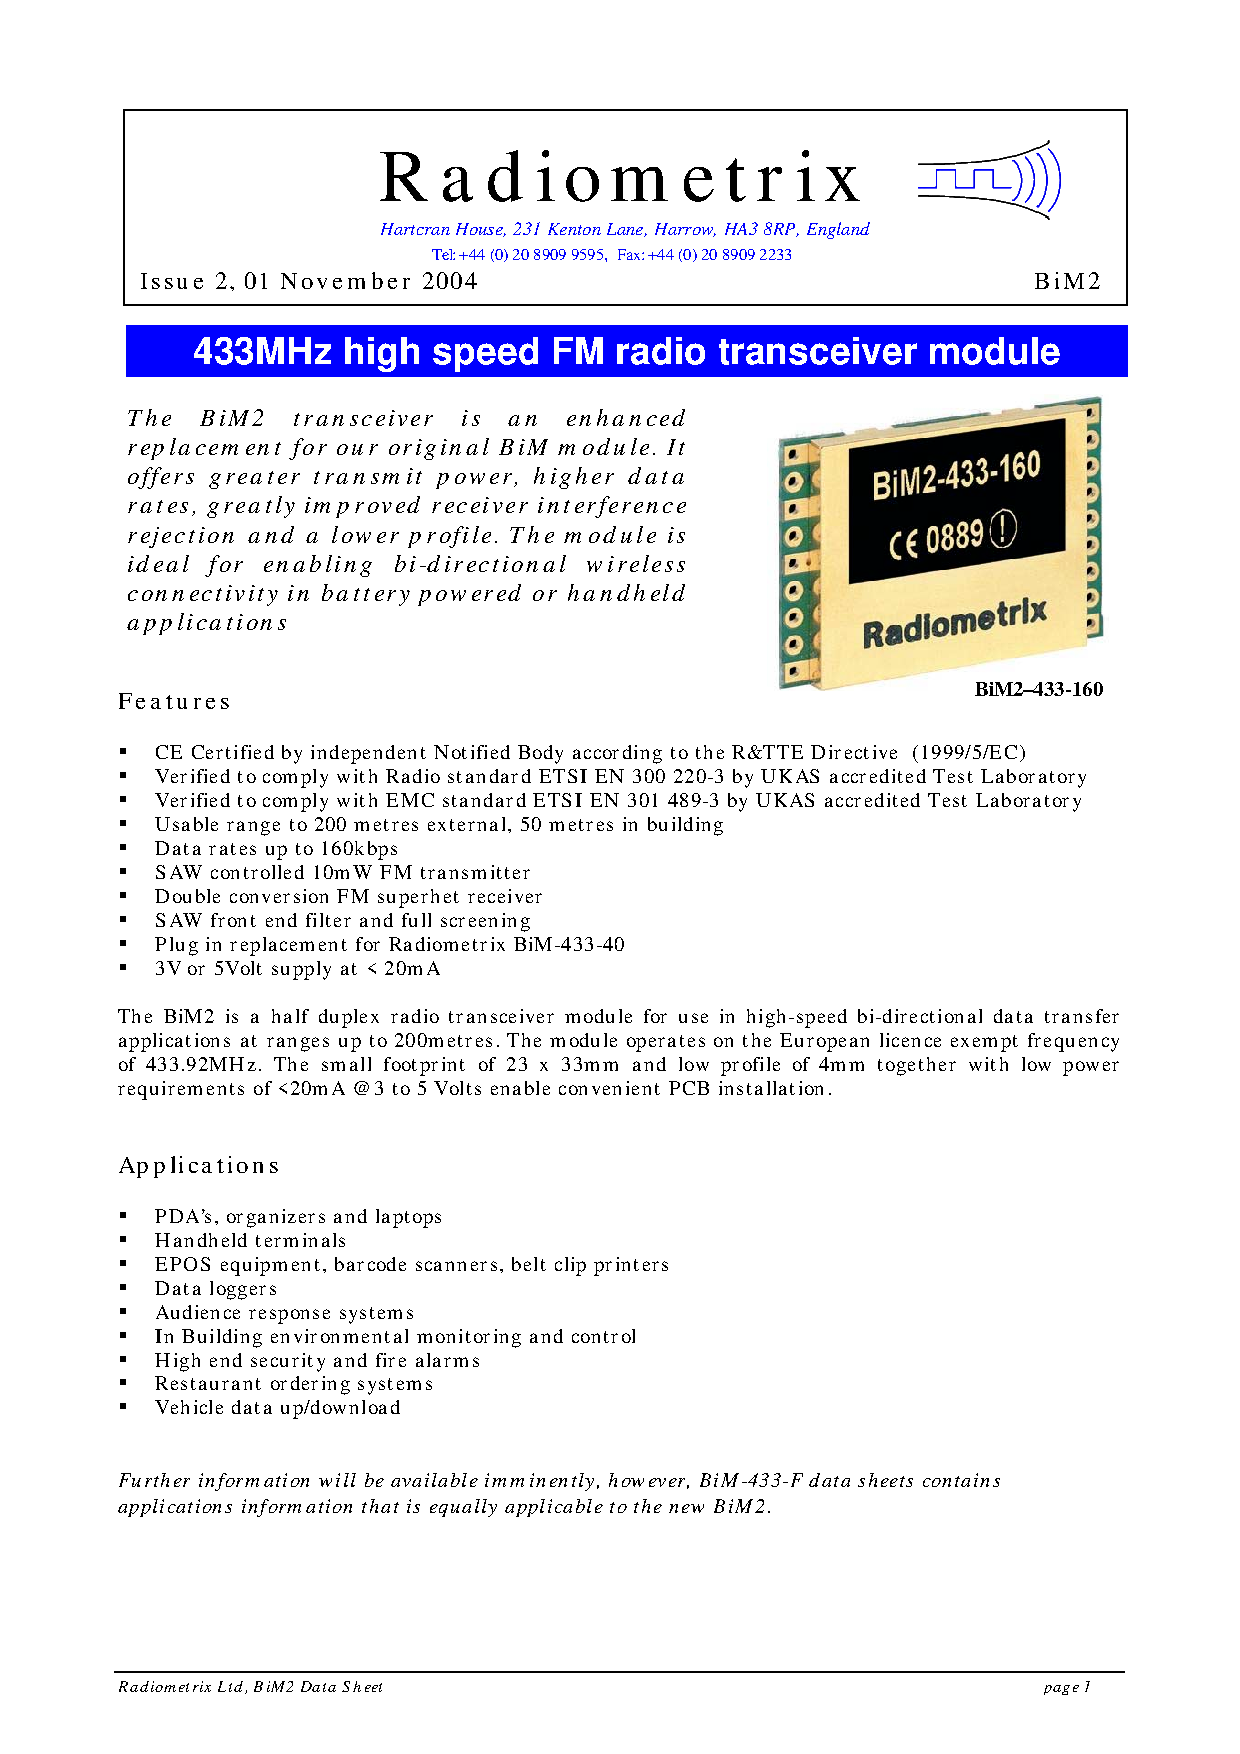
\includepdf[pages={1-}]{./datasheets/bim2.pdf}

\fi % End of datasheet section
\end{document}
